\cotefile{161-5}
\scanpage{17}
\mspage{131}
\begin{center}Sur les groupes de Galois attachés aux groupes $p$-divisibles\end{center}

spéciale aux groupes de dimension 1). On en déduit que \textit{$I$ est un sous-groupe ouvert de $G$}; je ne connais pas de démonstration directe de ce fait.

3) Le groupe $I$ possède deux filtrations naturelles $v$ et $w$, définies de la manière suivante:
\[
\begin{aligned}
v(g)&\geqslant n\Leftrightarrow(g-1)(T)\subset p^nT\,,\\
w(g)&\geqslant n\Leftrightarrow g\in I^n
\end{aligned}
\]
($I^n$ désigne le $n$-ème groupe de ramification de $I$, dans la notation supérieure, cf. [\textit{6}], chap. IV, \S~3).

Quelle relation y a-t-il entre $v$ et $w$? Si $e_K$ désigne l’indice de ramification absolu de $K$, est-il vrai que l’on a
\[
w=e_K\cdot v+O(1)\,?
\]
% Right bracket, with a middle stroke, spans the question and the following paragraph.
\margin{\handwritten{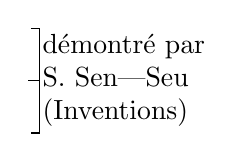
\begin{tikzpicture}[baseline=(n.center)]
\node[align=left,inner sep=0pt] (n) at (0,0) {démontré par\\S. \unsure{Sen|Seu}\\(Inventions)};
\draw ([xshift=-4pt,yshift=2pt]n.north west) -- ([xshift=-1pt,yshift=2pt]n.north west) -- ([xshift=-1pt,yshift=-2pt]n.south west) -- ([xshift=-4pt,yshift=-2pt]n.south west);
\draw ([xshift=-5pt]n.west) -- ([xshift=-1pt]n.west);
\end{tikzpicture}}}
Une question analogue se pose pour tous les groupes de Lie $p$-adiques qui sont des groupes de Galois.

\begin{center}\textbf{Bibliographie}\end{center}

[\textit{1}] \textsc{Chevalley}, C.: Théorie des groupes de LIE, II et III. Publ. Inst. Math. Univ. Nancago, Paris: Hermann 1951 et 1955.

[\textit{2}] \textsc{Lubin}, J.: One-parameter formal LIE groups over $p$-adic integer rings. Ann. of Maths. \textbf{80}, 464--484 (1964).

[\textit{3}] \textsc{Lubin}, J.: Finite subgroups and isogenies of one-parameter formal LIE groups. Ann. of Maths. \textbf{85}, 296--302 (1961).

[\textit{4}] \textsc{Mumford}, D.: Geometric invariant theory. Ergeb. der Math., Neue Folge, Bd. 34. Berlin, Heidelberg, New York, Springer 1965.

[\textit{5}] \textsc{Mumford}, D.: Families of abelian varieties. Algebraic groups and discontinuous subgroups. Proc. Symp. Pure Maths. \textbf{9}, A.M.S. (1966).

[\textit{6}] \textsc{Serre}, J-P.: Corps Locaux. Publ. Inst. Math. Univ. Nancago, VIII, Paris: Hermann 1962.

[\textit{7}] \textsc{Serre}, J-P.: LIE algebras and LIE groups. New York: Benjamin 1965.

[\textit{8}] \textsc{Serre}, J-P.: Résumé des cours 1965--66. Annuaire du Collège de France, 49--58, (1966--67).

[\textit{9}] \textsc{Tate}, J.: $p$-divisible groups, ce volume p. 158--183.
% archive sheet number: 16
\scanpage{18}
\begin{center}
{\Large EXTRAIT}

DE

L’ANNUAIRE DU COLLÈGE DE FRANCE

\rule{1.2cm}{0.4pt}

68\textsuperscript{e} ANNÉE

(1968-1969)

\rule{1.2cm}{0.4pt}

{\large RÉSUMÉ DES COURS DE 1967-1968}

\rule{1.8cm}{0.4pt}
\end{center}
% archive sheet number: 17
\scanpage{19}
\mspage{--- 47 ---}
\begin{center}
\textbf{Algèbre et géométrie}

M. Jean-Pierre \textsc{Serre}, professeur
\end{center}

Soit $\mathrm{K}$ un corps complet pour une valuation discrète, de corps résiduel $k$. On suppose que $\mathrm{K}$ est de caractéristique zéro et que $k$ est algébriquement clos de caractéristique $p$. Soit $\bar{\mathrm{K}}$ une clôture algébrique de $\mathrm{K}$, et soit $\mathrm{G}$ le groupe de Galois de $\bar{\mathrm{K}}$ sur $\mathrm{K}$. Soit $\mathrm{V}$ un espace vectoriel de dimension finie sur le corps $p$-adique $\mathbf{Q}_p$, et soit
\[
\varrho:\mathrm{G}\longrightarrow\operatorname{Aut}(\mathrm{V})
\]
un homomorphisme continu. On dit alors que $\mathrm{V}$ (ou $\varrho$) est une \textit{représentation $p$-adique} de $\mathrm{G}$.

Soit $\chi$ l’homomorphisme de $\mathrm{G}$ dans le groupe des unités $p$-adiques correspondant à l’action naturelle de $\mathrm{G}$ sur les racines de l’unité d’ordre une puissance de $p$. Soit $\mathrm{C}$ le complété de $\bar{\mathrm{K}}$. Si $\mathrm{V}$ est, comme ci-dessus, une représentation $p$-adique de $\mathrm{G}$, posons $\mathrm{V}_{\mathrm{C}}=\mathrm{C}\otimes\mathrm{V}$ (le produit tensoriel étant pris sur $\mathbf{Q}_p$) ; pour tout $n\in\mathbf{Z}$, soit $\mathrm{V}_{\mathrm{C}}^n$ le $\mathrm{K}$-sous-espace de $\mathrm{V}_{\mathrm{C}}$ formé des éléments $x$ tels que $\varrho(s)x=\chi(s)^nx$ pour tout $s\in\mathrm{G}$, et soit $\mathrm{V}_{\mathrm{C}}(n)=\mathrm{C}\otimes_{\mathrm{K}}\mathrm{V}_{\mathrm{C}}^n$. D’après un résultat de \textsc{Tate}, la somme directe des $\mathrm{V}_{\mathrm{C}}(n)$ s’identifie à un sous-espace vectoriel de $\mathrm{V}_{\mathrm{C}}$. On dit que $\mathrm{V}$ admet une \textit{décomposition de Hodge $p$-adique} (ou que $\mathrm{V}$ est un \textit{module de Hodge}) si ce sous-espace vectoriel est égal à $\mathrm{V}_{\mathrm{C}}$, autrement dit si l’on a :
\[
\mathrm{V}_{\mathrm{C}}=\sum_{n\in\mathbf{Z}}\mathrm{V}_{\mathrm{C}}(n).
\]

Soit $\mathrm{V}$ un tel module, soit $\mathrm{G}_{\mathrm{V}}=\varrho(\mathrm{G})$ le sous-groupe correspondant de $\operatorname{Aut}(\mathrm{V})$, et soit $\mathrm{H}_{\mathrm{V}}$ \textit{l’enveloppe algébrique} de $\mathrm{G}_{\mathrm{V}}$, autrement dit le plus petit sous-groupe algébrique (sur $\mathbf{Q}_p$) du groupe linéaire $\mathbf{GL}_{\mathrm{V}}$ dont le groupe des points contienne $\mathrm{G}_{\mathrm{V}}$.

Le sujet du cours a été l’étude du groupe $\mathrm{H}_{\mathrm{V}}$, et en particulier la démonstration des résultats suivants :
% archive sheet number: 18
\scanpage{20}
\mspage{--- 48 ---}
1) Le groupe $\mathrm{G}_{\mathrm{V}}$ est un sous-groupe \textit{ouvert} du groupe $\mathrm{H}_{\mathrm{V}}(\mathbf{Q}_p)$ des points de $\mathrm{H}_{\mathrm{V}}$ à coefficients dans $\mathbf{Q}_p$.

Il revient au même de dire que l’algèbre de Lie du groupe analytique $p$-adique $\mathrm{G}_{\mathrm{V}}$ est \textit{algébrique}, au sens de Chevalley.

2) La décomposition $\mathrm{V}_{\mathrm{C}}=\sum\mathrm{V}_{\mathrm{C}}(n)$ définit un homomorphisme
\[
h:\mathbf{G}_m/_{\mathrm{C}}\longrightarrow\mathbf{GL}_{\mathrm{V}}/_{\mathrm{C}}
\]
de groupes algébriques sur $\mathrm{C}$. Soit $\mathrm{H}_{\mathrm{V}}^{\unsure{\mathrm{O}|0|\circ}}$ la composante neutre de $\mathrm{H}_{\mathrm{V}}$, et soit $\mathrm{H}_{\mathrm{V}}^{\mathrm{O}}/_{\mathrm{C}}$ le sous-groupe de $\mathbf{GL}_{\mathrm{V}}/_{\mathrm{C}}$ déduit de $\mathrm{H}_{\mathrm{V}}^{\mathrm{O}}$ par extension des scalaires de $\mathbf{Q}_p$ à $\mathrm{C}$. Alors $\mathrm{H}_{\mathrm{V}}^{\mathrm{O}}/_{\mathrm{C}}$ \textit{contient le groupe} $h(\mathbf{G}_m/_{\mathrm{C}})$, image de $h$.

Lorsque de plus $\mathrm{G}_{\mathrm{V}}$ est \textit{résoluble}, on peut caractériser $\mathrm{H}_{\mathrm{V}}^{\mathrm{O}}$ comme \textit{le plus petit sous-groupe algébrique} $\mathrm{R}$ sur $\mathbf{Q}_p$ de $\mathbf{GL}_{\mathrm{V}}$ \textit{tel que} $\mathrm{R}/_{\mathrm{C}}$ \textit{contienne} $h(\mathbf{G}_m/_{\mathrm{C}})$ ; c’est l’analogue $p$-adique du \textit{groupe de Mumford-Tate}.

Il est probable que cette caractérisation de $\mathrm{H}_{\mathrm{V}}^{\mathrm{O}}$ vaut sans supposer $\mathrm{G}_{\mathrm{V}}$ résoluble ; on pourrait le prouver si l’on savait que $\mathrm{V}_{\mathrm{C}}=\mathrm{V}_{\mathrm{C}}(0)$ entraîne que $\mathrm{G}_{\mathrm{V}}$ est fini.
% slanted
\reversemarginpar
\margin{\handwritten{\shortstack[l]{ceci a été\\démontré par\\S. Sen (Annals)}\,$\left[\vphantom{\begin{matrix}1\\1\\1\end{matrix}}\right.$}}
\normalmarginpar

3) Lorsque $\mathrm{V}$ varie, les groupes $\mathrm{H}_{\mathrm{V}}$ forment un système projectif ; leur limite projective est un \textit{groupe proalgébrique} $\mathrm{H}$ sur $\mathbf{Q}_p$, muni d’un homomorphisme $h:\mathbf{G}_m/_{\mathrm{C}}\longrightarrow\mathrm{H}/_{\mathrm{C}}$. La catégorie des modules de Hodge est équivalente à celle des $\mathrm{H}$-modules de dimension finie ; si $\mathrm{H}^{\unsure{\mathrm{o}|\circ}}$ désigne la composante neutre de $\mathrm{H}$, le groupe $\mathrm{H}/\mathrm{H}^{\mathrm{o}}$ est le groupe de dimension zéro associé au groupe profini $\mathrm{G}$ ; le groupe $\mathrm{H}^{\mathrm{o}}$ ne change pas lorsqu’on remplace $\mathrm{K}$ par une extension finie.

4) Soit $\Theta$ le plus grand quotient commutatif du groupe proalgébrique $\mathrm{H}^{\mathrm{o}}$. Le groupe $\Theta$ est une limite projective de tores ; il ne dépend que de $p$ (mais pas de $\mathrm{K}$) ; on a :
\[
\Theta=\underset{\leftarrow}{\mathrm{lim.}}\,\mathrm{T}_{\mathrm{E}}
\]
où $\mathrm{E}$ parcourt l’ensemble des extensions finies de $\mathbf{Q}_p$.

(Si $\mathrm{E}$ est une extension de $\mathbf{Q}_p$ de degré $n$, on note $\mathrm{T}_{\mathrm{E}}$ le tore $\mathrm{R}_{\mathrm{E}}/_{\mathbf{Q}_p}(\mathbf{G}_m/_{\mathrm{E}})$ défini par $\mathrm{E}$ ; sa dimension est $n$, et $\mathrm{T}_{\mathrm{E}}(\mathbf{Q}_p)$ est canoniquement isomorphe à $\mathrm{E}^{*}$.)

Ce résultat est essentiellement équivalent à un théorème exposé par \textsc{Tate} dans le séminaire 1965/66. Il est intimement lié aux propriétés des « multiplications complexes formelles » des groupes $p$-divisibles.
% archive sheet number: 19
\scanpage{21}
\mspage{--- 49 ---}
5) Faisons maintenant l’hypothèse que $\mathrm{V}$ ne fait intervenir que les exposants 0 et 1, autrement dit que $\mathrm{V}_{\mathrm{C}}=\mathrm{V}(0)+\mathrm{V}_{\mathrm{C}}(1)$ ; posons
\[
n_{\unsure{\mathrm{o}|0}}=\dim_{\mathrm{C}}\mathrm{V}_{\unsure{\mathrm{C}|\dot{\mathrm{C}}}}(0)\ \text{et}\ n_1=\dim_{\mathrm{C}}\mathrm{V}_{\mathrm{C}}(1).
\]
(Le module $p$-adique attaché à un groupe $p$-divisible est de ce type, l’entier $n_1$ étant égal à la dimension du groupe.)

Supposons que $n_1=1$ et que $\mathrm{V}$ soit un $\mathrm{H}_{\mathrm{V}}^{\unsure{\mathrm{O}|0|\circ}}$-module simple. Alors le commutant de $\mathrm{H}_{\mathrm{V}}^{\mathrm{O}}$ dans $\operatorname{End}(\mathrm{V})$ est un corps commutatif $\mathrm{E}$ de degré fini sur $\mathbf{Q}_p$, et $\mathrm{H}_{\mathrm{V}}^{\mathrm{O}}$ est égal au groupe algébrique des $\mathrm{E}$-automorphismes de $\mathrm{V}$ ; il en résulte, conformément à ce qu’avaient conjecturé \textsc{Lubin} et \textsc{Tate}, que le groupe $\mathrm{G}_{\mathrm{V}}$ contient un sous-groupe \textit{ouvert} de $\operatorname{Aut}_{\mathrm{E}}(\mathrm{V})$.

Le cours s’est achevé par un essai de classification dans le cas $n_1>1$ (en supposant $\mathrm{V}$ absolument simple sur $\mathrm{H}_{\mathrm{V}}^{\mathrm{O}}$), basé sur le fait que $\mathrm{H}_{\mathrm{V}}^{\mathrm{O}}/_{\mathrm{C}}$ contient un tore de dimension 1 \textit{n’ayant que deux poids}.
% slanted
\margin{\handwritten{$\left.\vphantom{\begin{matrix}1\\1\end{matrix}}\right]$ voir à ce sujet le livre de T. Springer sur \unsure{les|ls} alg. de Jordan récemment paru chez Springer-Verlag}}

\begin{center}\textsc{Séminaire}\end{center}

Le séminaire a continué celui de 1965/66, relatif aux \textit{groupes $p$-divisibles}. Il a comporté neuf exposés : quatre par Michel \textsc{Raynaud} et cinq par John \textsc{Tate} (qui en avait fait dix en 1965/66).

Michel \textsc{Raynaud} a rappelé les notions préliminaires nécessaires : schémas en groupes finis, dualité de Cartier, quotients. Il a ensuite donné la définition des groupes $p$-divisibles, et montré leur interprétation comme groupes formels. Dans son dernier exposé, il a démontré le théorème fondamental, dû à \textsc{Tate}, qui affirme que, en inégale caractéristique, le passage de l’anneau des entiers au corps des fractions définit un foncteur \textit{pleinement fidèle} sur la catégorie des groupes $p$-divisibles. Il est possible que sa démonstration, différente de celle de \textsc{Tate}, puisse être adaptée au cas d’égale caractéristique.

Les exposés de John \textsc{Tate} ont eu pour thème le \textit{théorème de relèvement} des variétés abéliennes, autrement dit le fait que relever une variété abélienne revient à relever le groupe $p$-divisible correspondant (la caractéristique résiduelle étant égale à $p$). A Woods Hole, en 1964, \textsc{Tate} en avait donné une démonstration basée sur une certaine construction cohomologique. Dans le séminaire, il a proposé une autre méthode, où variété abéliennes et groupes $p$-divisibles n’interviennent que par les \textit{faisceaux} correspondants (pour des topologies d’\textsc{Artin-Grothendieck} convenables). Cette méthode, malgré des difficultés techniques qui n’ont pas été entièrement résolues, paraît plus naturelle que la précédente, et de portée plus générale.

\noindent{\footnotesize 4}
% archive sheet number: 20
\scanpage{22}
\mspage{--- 50 ---}
Un cas particulier intéressant est celui où la variété abélienne est \textit{ordinaire}, autrement dit a le maximum possible de points d’ordre $p$. Il existe alors un \textit{relèvement canonique} que l’on peut caractériser de diverses manières ; dans le cas des courbes elliptiques, ce relèvement avait été signalé en 1933 par H. \textsc{Hasse} (qui se plaçait à un point de vue quelque peu différent).

\begin{center}\textsc{Publications}\end{center}

H. \textsc{Bass}, J. \textsc{Milnor} et J.-P. \textsc{Serre}, \textit{Solution of the congruence subgroup problem for} $\mathrm{SL}_n$ $(n\geqslant 3)$ \textit{and} $\mathrm{Sp}_{2n}$ $(n\geqslant 2)$ (\textit{Publ. Math. I.H.E.S.}, n\textsuperscript{o} 33, 1967, p. 59-137).

J.-P. \textsc{Serre}, \textit{Local Class Field Theory} ; \textit{Complex Multiplication} (chap. VI et XIII de J. \textsc{Cassels} et A. \textsc{Fröhlich}, \textit{Algebraic Number Theory}, Acad. Press, New York, 1967).

--- \textit{Sur les groupes de Galois attachés aux groupes $p$-divisibles} (\textit{Proc. Conf. Local Fields}, Driebergen, 1966, Springer-Verlag, p. 118-131).

--- \textit{Commutativité des groupes formels de dimension} 1 (\textit{Bull. Sci. math.}, 91, 1967, p. 113-115).

--- \textit{Représentations linéaires des groupes finis} (Paris, Hermann, 1968).

--- \textit{Abelian $l$-adic representations and elliptic curves} (Notes rédigées avec la collaboration de W. \textsc{Kuyk} et J. \textsc{Labute}, W. A. Benjamin Publ., New York, 1968).

\begin{center}\textsc{Missions}\end{center}

Cours à McGill University, Montréal (septembre 1967).

Conférences à l’Université de Montréal (septembre 1967), à Haverford College (octobre 1967), à l’Institute for Advanced Study de Princeton (octobre-décembre 1967) et à l’Université de Grenoble (juin 1968).
% archive sheet number: 21
\scanpage{23}
\deleted{\unsure{Soit}} $K$ corps local d’inégales caractéristiques, corps résiduel $k$ de car. $p>0$ ($k$ parfait!), anneau d’entiers $V$, sous-$p$-anneau $W$ de corps résiduel $k$, corps des fractions $L$. On choisit une clôture algébrique $\bar K\deleted{\Omega}$ de $K$, son complété est $\Omega$.

\diagram{\begin{tikzcd}[ampersand replacement=\&,column sep=2pt,row sep=1pt]
L \& \subset \& K \& \subset \& \bar K \& \subseteq \& \Omega\\
\cup \& \& \cup \& \& \cup \& \& \cup\\
W \& \unsure{\in|\subset} \& V \& \subset \& \bar V \& \subset \& \widehat{\bar V}
\end{tikzcd}}

On pose
\[
\pi=\operatorname{Gal}(\bar K/K),\ \pi'=\operatorname{Gal}(\bar K/L)\,\ldots
\]
$\mathcal M_K=$ catégorie des \inserted{$\mathbb Q_p$-}faisceaux du type Hodge-Tate sur $K$ \inserted{($\otimes$-catégorie sur $\mathbb Q_p$)}

$\mathcal M_K^+=\underset{\longrightarrow}{\lim}\mathcal M^{(n)}$, ss-catégorie des objets ``effectifs'' i.e. avec \deleted{\unsure{la graduation|graduation}} $\operatorname{gr}(M_\Omega)$ à degrés positifs

$\mathcal M_K^{(\unsure{n|1})}=\bigl\{$ \deleted{\unsure{ss-}}catégorie pleine de $\mathcal M$ formée des $M$ avec $\operatorname{gr}M_\Omega$ à degrés $0$ et $1$

$\widetilde{\mathrm{BT}}_{\deleted{\unsure{K}}V}$ catégorie des BT à isog. près \uline{sur $V$}

Foncteur pl. fid (par Tate)
\[
\widetilde{\mathrm{BT}}_V\lhook\joinrel\longrightarrow\mathcal M_K^{(\unsure{1|n})}
\]
\margin{on identifie $\widetilde{\mathrm{BT}}_V$ à ss-catégorie pleine de $\mathcal M_K^{(1)}$}

$\mathcal M_{\deleted{\unsure{K+|K}}}^{\mathrm{BT}}\subset\mathcal M_K$ $\otimes$-\deleted{\unsure{ss-}}catégorie Tannakienne engendrée par $\mathcal M_K^{(1)}$

\[
T_p^\Omega=T_p:\mathcal M_K\longrightarrow\deleted{\unsure{\operatorname{Rep}(\pi,\mathbb Q_p)}}\,\operatorname{Mod\,f}(\mathbb Q_p)
\qquad\text{foncteur fibre en }\Omega
\]
\[
G^\Omega=G^{\deleted{\unsure{\Omega}}}=\operatorname{Aut}(T_p)
\qquad\text{pro-groupe alg. sur }\mathbb Q_p
\]
\[
\pi\xrightarrow{\rho}G(\mathbb Q_p)\qquad
\begin{aligned}
&G\text{ est l’enveloppe algébrique de }\pi\\
&(\mathrm{NB}\quad G/G^{\unsure{\circ|0}}\ \text{non tordu})
\end{aligned}
\]

Pour $M\in\operatorname{Ob}\mathcal M$,
\[
G_M=\operatorname{Im}\bigl(G\longrightarrow\underline{\operatorname{Aut}}_{\mathbb Q_p}(T_p(M))\bigr)\subset\underline{\operatorname{Aut}}_{\mathbb Q_p}(T_p(M))
\]
\[
\bigl(\pi_{\deleted{\unsure{M}}}\xrightarrow{\rho_M}G_M(\mathbb Q_p)\quad\ldotp\ldotp\ldotp\ldotp\ldotp\ \bigr)
\]

\diagram{\resizebox{\linewidth}{!}{$\begin{array}{lllll}
\substack{\text{structure}\\\text{sur }(\Omega,\pi)}
&\begin{tikzcd}[ampersand replacement=\&,row sep=0pt,column sep=3pt] \&G^{!}_{\Omega}\\G_{m_\Omega}\arrow[ur,"{\unsure{j|J}^{!}}"]\&\end{tikzcd}
&\substack{\unsure{\Phi|P|\mathfrak{P}}\\\text{avec section }e\\\text{sur }\Omega\\\text{\unsure{pas invariante|non invariante} sous }\pi}
&G_\Omega&\\[4pt]
\text{id}
&\begin{tikzcd}[ampersand replacement=\&,row sep=0pt,column sep=3pt] \&G^{\mathrm{Hdg}}_{\Omega}\\G_{m_\Omega}\arrow[ur,"{j_\Omega}"]\&\end{tikzcd}
&Q_\Omega=\unsure{\mathcal T|\tau}\mathbin{\wedge}_{G_{m_\Omega}}\Phi&G_\Omega&\\[4pt]
\substack{\text{par descente}\\\text{sur }K}
&\begin{tikzcd}[ampersand replacement=\&,row sep=0pt,column sep=3pt] \&G^{\mathrm{Hdg}}_{K}\\G_{m_K}\arrow[ur,"{j_K}"]\&\end{tikzcd}
& Q_K&G_K&T_{\mathrm{Hdg}}^{\deleted{\unsure{K}}}(M)=Q_K\mathbin{\wedge}_G M_K
\end{array}$}}
\margin{$\bigl[\mathcal T\deleted{\unsure{=}}\inserted{=\mathcal T^\Omega}$ $G_{m_\Omega}$-tor, sur $(\Omega,\pi)$ associé à $T_p(\Omega^\times)\otimes_{\mathbb Z_p}\Omega$ $\bigr]$}

Pour $M\in\operatorname{Ob}\widetilde{\mathrm{BT}}_V$, on a \deleted{\unsure{sur} $T_{\mathrm{Hdg}}(M)$} un

a) Un $\deleted{\unsure{K}}L$-vectoriel \deleted{\unsure{filtré}} $T_{\unsure{\mathrm{dR}|\mathrm{DR}|\mathrm{cr}}}(M)$ \deleted{et un isom}

\deleted{$\operatorname{gr}T_{\mathrm{DR}}(M)_K\simeq T_{\mathrm{Hdg}}(M)$}
% archive sheet number: 22
\scanpage{24}
b) Une \deleted{\unsure{donnée de|donnée}}\inserted{structure} de F-\inserted{iso}cristal sur $T_{\mathrm{cr}}(M)$

c) Une filtration de $T_{\mathrm{DR}}(M)=T_{\mathrm{cr}}(M)\otimes_K L$

d) Un isomorphisme
\[
\operatorname{gr}(T_{\mathrm{DR}}(M))\simeq T_{\mathrm{Hdg}}(M)
\]

ces données étant fonctorielles en $M\in\operatorname{Ob}\widetilde{\mathrm{BT}}_{\unsure{V|K}}$

\uline{Question}\qquad Peut-on prolonger ces données à $\mathcal M^{\mathrm{BT}}$, \deleted{\unsure{? A-t-on}}

\noindent\begin{tabular}{|p{0.88\linewidth}}
avec $T_{\mathrm{cr}}$ un $\otimes$-foncteur, \unsure{le|la} structure b) \unsure{compatible|compatibles} avec $\otimes$\inserted{ et Hom}, c) et d) aussi. A-t-on unicité de $T_{\mathrm{cr}}$ prolongé, à isom unique près ?
\end{tabular}
% archive sheet number: 23
\scanpage{25}
1) gr. alg $\boxed{G}$ sur $\mathbb Q_p$

2) hom continu \(\boxed{\rho:\pi\unsure{\mathbin{-}|\longrightarrow}G(\mathbb Q_p)}\)

d’où $G_\Omega^{!}\mathbin{-}\unsure{Q|\Phi|\mathfrak{P}}_\Omega^{!}\mathbin{-}G_\Omega$

% slanted
\reversemarginpar
\margin{unique\,$\left\{\vphantom{\begin{matrix}1\\1\\1\\1\end{matrix}}\right.$}
\normalmarginpar
3) \(\boxed{G_{m_\Omega}\xrightarrow{\unsure{j|J}^{!}}G_\Omega^{!}}\) \qquad d’où
\diagram{\begin{tikzcd}[ampersand replacement=\&,row sep=3pt,column sep=5pt]
\&Q_\Omega=\unsure{\mathcal T|\tau}\mathbin{\wedge}_{G_{m_\Omega}}Q_\Omega^{!}\arrow[dl,dash]\arrow[dr,dash]\&\\
G_\Omega^{\prime\prime}=\mathcal T\bigl(\mathbin{\wedge}^{\ast}_{G_{m_\Omega}}(G_\Omega^{!},\unsure{i^{-1}|\mathrm{int}})\bigr)\&\&G_\Omega\\
j_\Omega:G_m\longrightarrow G_\Omega^{\prime\prime}\&\&
\end{tikzcd}}
\deleted{4)}

4) \(\boxed{Q_L\ \text{sous }G_L}\) descendant $Q_\Omega$ sous $G_\Omega$
\[
U_L^{\prime\prime}\subset G_L^{\prime\prime}\mathbin{-}Q_L\mathbin{-}G_L,\quad
j_L:G_{m_L}\unsure{\longrightarrow|\mathbin{-}}G_L^{\prime\prime}
\]

5) \deleted{\unsure{Un ensemble} $\boxed{\Delta}$ d’opérations \inserted{$\rho$} de $\Gamma$ $(\supset\pi)$ sur $Q_\Omega$ \unsure{compatibles} \illegible{2} prolongeant celle de $\pi$, \inserted{d’où $\Gamma\longrightarrow G_L^{\prime\prime}(\unsure{\Omega|L})=G_\Omega^{\prime\prime}(\Omega)$} comp. à \unsure{une action|son action|celle} de $\Gamma$ sur $\Omega$.

tel que si $\rho$ est stable par \unsure{les|les autres} formant orbite sous $U_L^{\prime\prime}(L)$ opérant par (pour $u\in U_L^{\prime\prime}(L)$)
\[
(u.\rho)(\unsure{\gamma})=\tau(u)\bigl(\rho(\gamma)\bigr)\tau(u)^{-1}=(\unsure{\operatorname{int}\tau(u)}).\rho(\gamma)
\]
i.e. $u\unsure{\mapsto|\mathbin{-}|\mathbin{.}}\rho=\operatorname{int}\tau(u)\rho)$

[ NB si $u.\rho=\rho$ i.e. $\tau(u),\rho$ commutent : \unsure{$\tau(u)$} pour \unsure{tout} ]}

Un torseur (ensembliste) \inserted{à droite} $R_0\inserted{\Delta}$ sous $U_L^{\prime\prime}(L)$, et un $U_L^{\prime\prime}(L)$-\uline{hom de}
\[
\left[\begin{aligned}
\rho:\Delta\longrightarrow{}&\text{Op. de }\Gamma\text{ sur }(\Omega,Q_L,G_L)\\
&\text{qui sont compatibles avec}\\
&\text{\deleted{\unsure{l’}}l’op qu’on a de }\Gamma\text{ sur }\Omega,\\
&\text{et celle de }\pi\unsure{\subset|\in}\Gamma\text{ sur }Q_L\ldots
\end{aligned}\right.
\]
lorsque on fait opérer $U_L^{\prime\prime}(L)$ \inserted{à droite} sur le deuxième ens. par
\[
u.\alpha=\tau(\alpha)^{-1}u\tau(\alpha)^{\deleted{\unsure{-1}}}
\]
% archive sheet number: 24
\scanpage{26}
1) groupe Alg. $\boxed{G}$ sur $\mathbb Q_p$. (Il dépend en fait du choix de $\Omega$. cf plus bas 2\textsuperscript{o})

2) Hom \(\boxed{\rho:\pi\longrightarrow G(\mathbb Q_p)}\)

[ L’op. de $\pi=\operatorname{Aut}_L(\Omega)$ sur $G=G^{(\Omega)}$ est donnée par $\gamma\to\operatorname{int}(\rho(\gamma))$ ]

\deleted{3)} On fait opérer $\pi$ sur $G_\Omega$ \uline{diagonalement}, soit $G_\Omega^{!}$

3) Hom \(\boxed{j_{\deleted{\unsure{s}}}^{!}:G_{m_\Omega}\longrightarrow G_\Omega^{!}}\) \qquad inv. par $\pi$
\reversemarginpar\margin{$G_\Omega$\quad \unsure{1|!}}\normalmarginpar

On appelle $\deleted{\unsure{T_p}}\inserted{S_\Omega}(1)$ \deleted{\unsure{$T$}} le \deleted{\unsure{rep}} $\Omega$-module inversible $T_p(\Omega)^{\unsure{\times|\ast}}\otimes_{\mathbb Z_p}\Omega$ avec op. diagonale de $\pi$, \deleted{\unsure{associé}} et $\unsure{\mathcal T|\tau}_\Omega$ le $G_{m_\Omega}$ torseur associé. Posons

\deleted{$\mathcal T\mathbin{\wedge}_{\unsure{G_m}}^{\unsure{\Phi|\mathfrak{P}}}G_{m_\Omega}\quad G_{m_{\unsure{p}}}(\Omega)\quad\unsure{Q_\Omega}\quad\mathcal T\mathbin{\wedge}_{G_{m_\Omega}}\unsure{\Phi|\mathfrak{P}}_\Omega$}
\inserted{$Q_\Omega=\mathcal T\mathbin{\wedge}\unsure{\Phi|P|\mathfrak{P}}$} torseur \inserted{à dr} sous $G_\Omega$ à droite, à gauche est un \uline{$G_\Omega^{!}$ tordu} par $\mathcal T$, soit \tikz[baseline=(x.base)]{\node[draw,ellipse,inner sep=1pt](x){$G_\Omega^{\prime\prime}$};}.

[ correspondant au foncteur fibre \inserted{(gradué)} sur $\operatorname{Rep}(G)$
\[
G_{m_\Omega}\xrightarrow{j_\Omega^{\unsure{\prime\prime|\ast}}}G_\Omega^{\prime\prime}
\qquad M\to\sum\operatorname{gr}^{i}_{j}(M_\Omega)\otimes S_\Omega(-i)=\mathrm{Hdg}_\Omega(M)
\]

\unsure{$\subset$} \uline{Axiome} Le \deleted{foncteur}\inserted{torseur} $Q_\Omega$ \deleted{\unsure{sous}} se descend à $L$ en un $G_L$-torseur $Q_L$

\begin{center}\tikz[baseline=(x.base)]{\node[draw,ellipse,inner sep=3pt](x){$Q_L\quad G_L$};}\end{center}

(unique à isom unique près)

en un $G_L^{\prime\prime}$, et
\[
G_{m_L}\xrightarrow{j_L}G_L^{\prime\prime}
\]
Correspond à fct fibre gradué $\mathrm{Hdg}_L$

\margin{\uline{NB} Un $j$ satisfaisant ces conditions est unique. Signifie que les $M_\Omega^{\deleted{\unsure{0}}}$ \uline{sont de Hodge} Du moins si}

\noindent\rule{\linewidth}{0.4pt}

\textcircled{\unsure{1|a|2\textsuperscript{o}}} Il y a deux foncteurs fibres de $\operatorname{Rep}(G)$ dans $\operatorname{Mod}(\Omega,\pi)$

a) $M\longrightarrow M_\Omega$ opérations \unsure{provenant|par transport} des op. ordinaires de $\pi$ sur $\Omega$

b) $M\unsure{\longrightarrow|\mathbin{-}|\mapsto}M_\Omega^{!}$ opérations diagonales

- foncteurs $T_{\unsure{p\Omega|G\Omega|p,\Omega}}$ et $T_{p\Omega}^{!}$

\deleted{Après oubli des op.} On \unsure{a} alors un \deleted{\unsure{$(\Omega,\pi)$-}}torseur \inserted{à droite} sur $(\Omega,\pi)$ du groupe $G_\Omega$, soit $\Phi_\Omega$, donné par le 1-cocycle $\rho:\pi\unsure{\longrightarrow|\mathbin{-}}G(\mathbb Q_p)\subset H^0(\Omega,\pi\deleted{\unsure{G}},G_\Omega)=G(\unsure{L|k|\Omega})$. Le \deleted{groupe}\inserted{$(\Omega,\pi)$-} $\underline{\operatorname{Aut}}_{G_\Omega,\pi}(\Phi)$ est $G_\Omega^{!}$.
% archive sheet number: 25
\scanpage{27}
4) Soit \tikz[baseline=(x.base)]{\node[draw,ellipse,inner sep=1pt](x){$U_L^{\prime\prime}\subset G_L^{\prime\prime}$};} \uline{défini} par $j_L$. On a un torseur \inserted{à droite} \unsure{can|sur|canonique} (\unsure{ici|i.e.|mais} trivial) \(\boxed{R_L\ \text{sous } U_L^{\prime\prime}}\), d’où \unsure{le|$L$-} foncteur fibre filtré
\[
\mathrm{DR}_L(M)=\deleted{\unsure{T_p(M)_L}}\bigl(R_L\mathbin{\wedge}_{U_L^{\prime\prime}}Q_L\bigr)\mathbin{\wedge}_{G_L}T_p(M)_L
\]

\deleted{5)} Le foncteur fibre $\mathrm{DR}_L(M)$ correspond au $G_L$-tors. à dr.
\[
\tikz[baseline=(x.base)]{\node[draw,ellipse,inner sep=2pt](x){$R_L\mathbin{\wedge}_{U_L^{\unsure{\prime|\prime\prime}}}Q_L=P_L$};}
\]
Soit $G_L^{\prime\prime}=\underline{\operatorname{Aut}}(P_L)$ \qquad ($G_L^{\prime\prime}\simeq G_L^{\prime}$ non \unsure{canoniqt|canonique!|canoniquement})

\reversemarginpar\margin{$\left\{\vphantom{\begin{matrix}1\\1\\1\\1\end{matrix}}\right.$}\normalmarginpar
5) \uline{Structure de descente} de $L$ à $K$ \uline{sur le torseur} $P_L$, d’où
\[
G^{\prime\prime}\qquad P_K\qquad G_K
\]

6) $G_K$-Isom donné
\[
P_K\simeq P_K^{(\unsure{f|F|\sharp})}
\]

On peut formuler ensemble 5) et 6) en regardant
\[
P_{\deleted{\unsure{K}}\Omega}=R_L^{\deleted{\unsure{\leftarrow}}}\mathbin{\wedge}_{\deleted{\unsure{G}}U_\Omega^{\prime\prime}}Q_{\Omega}^{\prime\prime}=R_L\mathbin{\wedge}_{U_\Omega^{\prime\prime}}
\]
et en déclarant que l’ext. $\Gamma$ de $\mathbb Z$ par $\widetilde\pi=\operatorname{Gal}(\unsure{\bar K/K|\bar k/k|\bar K/\widetilde K})$ (qui contient $\pi\subset\Gamma$) \uline{opère} sur $P_\Omega$ en prolongeant l’op. qu’on a déjà sur $\pi$.
% archive sheet number: 26
\scanpage{28}
On a donc une \uline{extension}
\[
1\longrightarrow G'_S(S)\unsure{\longrightarrow|\mathbin{-}}\unsure{\mathcal E|E}\longrightarrow\Gamma\longrightarrow1\mathbin{\unsure{-|\longrightarrow}}\unsure{0|\circ|\ldotp}
\tag*{($\mathcal E$)}
\]

\deleted{Supposons que $\inserted{\pi}\pi\unsure{\in|\subset}\Gamma$ opère sur}

Les \uline{sections} de celle-ci sont les structures de torseur \unsure{sous|sur} $(S,\Gamma;G_S)$ sur $Q_S$ qui prolongent sa structure de Tor. sur $(S,G_S)$.

Si on a une telle section, on en déduit une opération de $\Gamma$ sur $G'_S(S)$ (qui en fait provient de son opération sur $G'_S$ lui-\unsure{=|même} !) et les autres sections correspondent aux 1-cocycles de $\Gamma$ à valeurs dans $G'_S(S)$. \deleted{Les}\inserted{L’ens $\Gamma(\mathcal E)$ des} sections \unsure{forment|forme} \deleted{\illegible{1}} un ens où $G'_S(S)$ opère (autom. intérieurs) et deux \deleted{\unsure{objets sont}} $\Gamma(\unsure{C|\mathcal E})$ sont \inserted{conjugués ssi le 1-cocycle faisant passer de l’un à l’autre est \unsure{``trivial''|réduit|cohom. à|coh. à} 1} Si on a un sous-groupe $\pi\subset\Gamma$ et une section $\alpha_0:\pi\longrightarrow\mathcal E$ partielle, on peut s’intéresser à l’ens des $g'\in G'_S(\unsure{S|1|L})$ qui la fixent, c’est \unsure{l’ens} des éléments de $G'_S(S)$ fixés par $\pi$ (y opérant comme de juste) $G'_S(S)^\pi\,(=\!G'_L(L))$. Les sections $\alpha$ qui prolongent $\alpha_0$ sont donc telles que $G'_S(S)^\pi$ y opère, Si on a
% archive sheet number: 27
\scanpage{29}
% One long oblique stroke passes through the upper text and runs into the
% gutter between the lower diagrams. Its scope as a cancellation is uncertain.
\deleted{un tel $\alpha$, les autres $\beta$ s’en déduisent par les 1-cocycles qui sont \uline{triviaux sur} $\pi$,
\[
\left\{\begin{aligned}
\varphi(\gamma\gamma')&=\varphi(\gamma)\,{}^\gamma\varphi(\gamma')\\
\varphi(\pi)&=\{e\}
\end{aligned}\right.
\]
\uline{Question}\qquad Est-il vrai que les $\alpha$ qui prolongent $\alpha_0$ sont \unsure{conj.|can.} i.e. conjugués sous $G'_S(S)$ ?

il suffirait de savoir que (pour une telle section fixée) $H^1(\Gamma,G'_S(S))\unsure{\longrightarrow|\mathbin{-}}H^1(\pi,G'_S(S))$ est injectif (ou \unsure{fblt|fbt|plutôt} injectif, i.e. noyau unité)

Si oui, les solutions cherchées forment un \deleted{torseur}\inserted{espace homogène} sous $G'_S(S)^\pi\ ( =G'_L(L))$}

\noindent\rule{0.38\linewidth}{0.4pt}

$H$

\[
\mathbb Q_p\mathbin{-}K
\qquad\qquad
T_K(\deleted{\unsure{K}})=\prod_{K/\mathbb Q_p}G_m
\]
\[
\prod_{\unsure{o|O|\sigma}/\mathbb Z_p}G_{\deleted{\unsure{M}}m}
\]
\diagram{\begin{tikzcd}[ampersand replacement=\&,row sep=11pt,column sep=10pt]
\& \& {}\arrow[r] \& T_{o_K}\arrow[r] \&\mathbb Z\arrow[r]\&0\\
\&0\arrow[r]\&g_{\unsure{o|0|\sigma}}\arrow[r]\&N\arrow[r]\arrow[ur,phantom,"{\text{\scriptsize Modèle de Néron de }g_K}" description]\&\mathbb Z_o\arrow[r]\&0\\
\unsure{m|u}\&0\arrow[r]\&g_o\arrow[r]\arrow[u,Rightarrow]\&\widetilde N\arrow[r]\arrow[u]\&\mathbb Z_o\arrow[r]\arrow[u]\&0\\
\unsure{m}\otimes_o K\&0\arrow[r]\&g_K\arrow[r]\&\widetilde N_K\arrow[r]\&\mathbb Z_K\arrow[r]\&0\\
\rotatebox{90}{$=$}\&\&\&\rotatebox{90}{$\simeq$}\&\&\\
K\&\&\&g_K\times\mathbb Z_K\&\&
\end{tikzcd}}

\diagram{\begin{tikzcd}[ampersand replacement=\&,column sep=small,row sep=8pt]
\&0\&\&0\\
\&\mathbb Z\arrow[u]\&\&\mathbb Z\arrow[u]\\
\&T_K(\mathbb Q_p)\simeq K^{*}\arrow[u]\&\unsure{m|u}\&{}\arrow[u]\\
\&o_K^{*}\arrow[u]\&\&\\
\&0\arrow[u]\&\&\\
\Gamma(N)\arrow[rr,"\sim"]\&\&\Gamma(g)=K^{*}\arrow[ddll,"{\pi}"']\&\\
\Gamma(\widetilde N)\arrow[u,"{\unsure{2|?|{\sim}}}"]\arrow[d,hook]\&\&\&\\
\Gamma(\widetilde N_K)\&\&\&\\
\rotatebox{90}{$\simeq$}\&\&\&\\
K^*\times\mathbb Z\&\&\&
\end{tikzcd}}
% archive sheet number: 28
